\chapter{Results}\label{final}

\section{Anomaly detection}

Using Isolation Forest we have performed anomaly detection to detect the faulty datapoints in the datasets. The 2D and 3D visualizations from t-SNE are as follows:

\begin{figure}
\makebox[\textwidth][c]{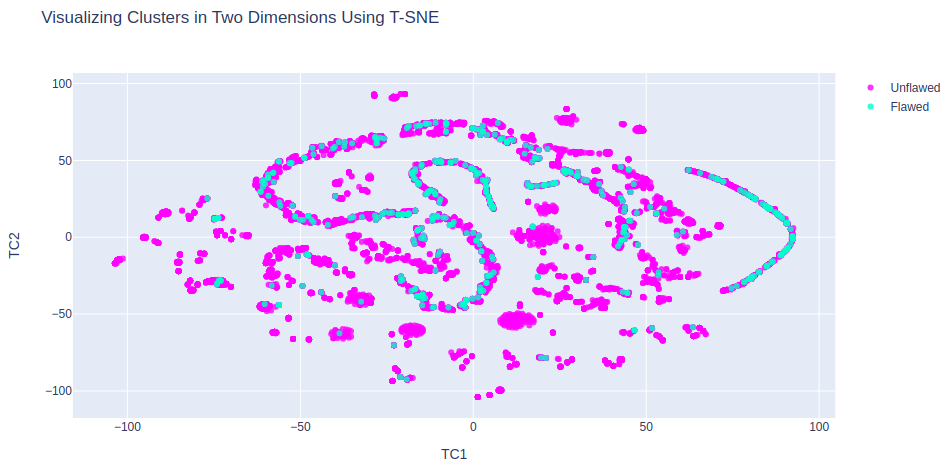
\includegraphics[width=0.8\textwidth]{others/2d_tsne.png}}%
  \caption{2D visualization}
  \label{fig:key}
\end{figure}

\begin{figure}
\makebox[\textwidth][c]{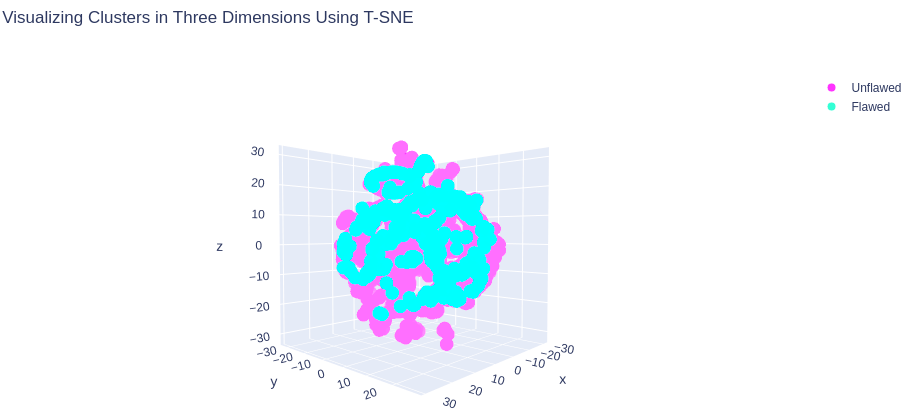
\includegraphics[width=0.8\textwidth]{others/3d_tsne.png}}%
  \caption{3D visualization}
  \label{fig:key}
\end{figure}

From the visualizations, it became clear that extensive feature reduction would not help in detecting the faulty datapoints. So, we proceeded without any feature selection. 
The datasets taken were initially labelled, so we found out the percentage of the faulty datapoints which came out to be 4.71 \% and plotted the distribution of the labels before removing the labels. The plot obtained is: 

\begin{figure}
\makebox[\textwidth][c]{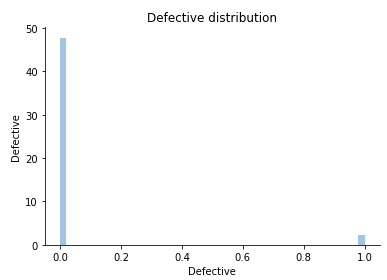
\includegraphics[width=0.8\textwidth]{others/defect_distribution.png}}%
  \caption{Distribution of labels}
  \label{fig:key}
\end{figure}

After applying the Isolation Forest model, we have obtained the Accuracy of the model by obtaining true positive, true negative and all samples count in the predictions. The formula for accuracy used is:

\[\frac{True Positive + True Negative}{All Samples}\] 

\section{Deep Learning Regression}
We performed 32 experiments without any feature selection and with three different feature selection techniques:
 \begin{itemize}
     \item Singular value Decomposition with 10 and 15 components
     \item Principal component analysis with 10 and 15 components
     \item Information Gain
 \end{itemize}
and each of SVD and PCA with two different number of components: 10 and 15.
Min Max scaling preprocessing was performed on the datasets before running all the models. The predictions obtained by all the models were rounded off to nearest integers. We used MSE as the loss function for all the models
We have developed 9 different models and tried 3 different architectures of LSTM, 3 different architectures of RNN and single architecture each of GRU, ANN and CNN.

\subsection{ANN}
The schematics of the ANN model designed is visualized as follows:

\begin{figure}
\makebox[\textwidth][c]{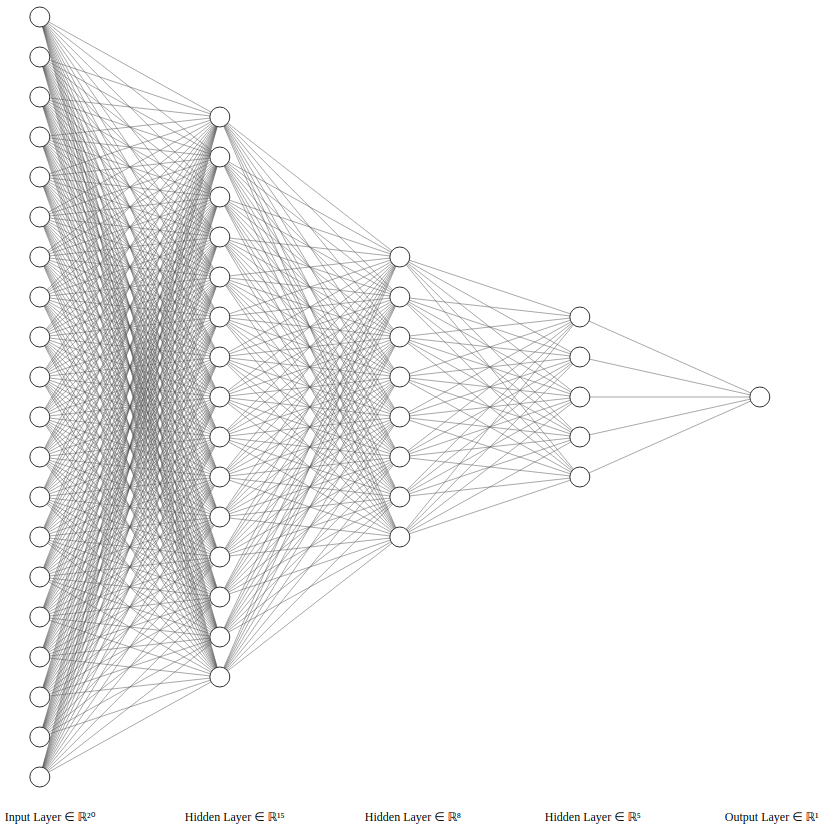
\includegraphics[width=0.8\textwidth]{others/nn.png}}%
  \caption{ANN Architecture}
  \label{fig:key}
\end{figure}
 
 The performance results are as follows:
 
%Please add the following packages if necessary:
%\usepackage{booktabs, multirow} % for borders and merged ranges
%\usepackage{soul}% for underlines
%\usepackage[table]{xcolor} % for cell colors
%\usepackage{changepage,threeparttable} % for wide tables
%If the table is too wide, replace \begin{table}[!htp]...\end{table} with
%\begin{adjustwidth}{-2.5 cm}{-2.5 cm}\centering\begin{threeparttable}[!htb]...\end{threeparttable}\end{adjustwidth}
\begin{table}[!htp]\centering
\caption{ANN Model results}\label{tab: }
\scriptsize
\begin{tabular}{lrrrrrr}\toprule
Feature Selection &No. of components &FPA &CLC &Train Loss at last epoch(MSE) &Test Loss(MSE) \\
\textbf{N/A} &\textbf{N/A} &\textbf{0.47545615} &\textbf{0.48384327} &\textbf{0.555} &\textbf{1.1668} \\\midrule
SVD &10 &0.47456595 &0.48294193 &0.385 &0.907 \\
SVD &15 &NAN &NAN &3.5 &0.3652 \\
PCA &10 &NAN &NAN &3.5 &0.3652 \\
PCA &15 &0.4627341 &0.47109878 &0.2115 &0.8144 \\
\bottomrule
\end{tabular}
\end{table}
 
Observing the results, we can see that the FPA and CLC is obtained to be NAN for two of the experiments. This situation is encountered when all the predictions i.e the number of bugs in the testing data come out to be zero after rounding off. This is an unwanted result. We also see that the best FPA and CLC are obtained when no feature selection technique is applied.

\subsection{GRU}
The schematics of the GRU model designed is visualized as follows:

\begin{figure}
\makebox[\textwidth][c]{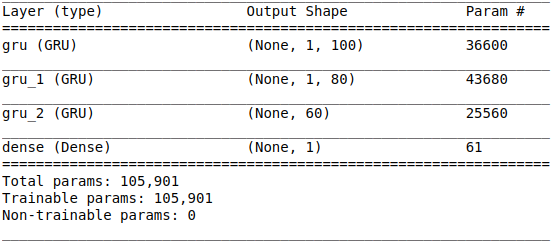
\includegraphics[width=0.8\textwidth]{others/gru_summary.png}}%
  \caption{GRU Architecture}
  \label{fig:key}
\end{figure}

Oversampling and SMOTE were applied to all the experiments involving the GRU model also. The performance results are as follows:
 
%Please add the following packages if necessary:
%\usepackage{booktabs, multirow} % for borders and merged ranges
%\usepackage{soul}% for underlines
%\usepackage[table]{xcolor} % for cell colors
%\usepackage{changepage,threeparttable} % for wide tables
%If the table is too wide, replace \begin{table}[!htp]...\end{table} with
%\begin{adjustwidth}{-2.5 cm}{-2.5 cm}\centering\begin{threeparttable}[!htb]...\end{threeparttable}\end{adjustwidth}
\begin{table}[!htp]\centering
\caption{GRU Model results}\label{tab: }
\scriptsize
\begin{tabular}{lrrrrrr}\toprule
Feature Selection &No. of components &FPA &CLC &Train Loss at last epoch(MSE) &Test Loss(MSE) \\
N/A &N/A &0.48528624 &0.49368343 &0.9214 &1.3261 \\\midrule
SVD &10 &0.48289812 &0.49128413 &0.7384 &1.0185 \\
SVD &15 &0.47688892 &0.4852823 &0.6949 &1.2748 \\
\textbf{PCA} &\textbf{10} &\textbf{0.49431464} &\textbf{0.5027083} &\textbf{0.7483} &\textbf{1.1861} \\
PCA &15 &0.4928466 &0.5012389 &0.7455 &1.1761 \\
\bottomrule
\end{tabular}
\end{table}
 
Observing the results, we see that the best FPA and CLC are obtained when PCA is applied and 10 components were taken for training the model and the least FPA and CLC are obtained when SVD is applied and 15 components were taken for training the model.

\subsection{CNN}
The schematics of the CNN model designed is visualized as follows:

\begin{figure}
\makebox[\textwidth][c]{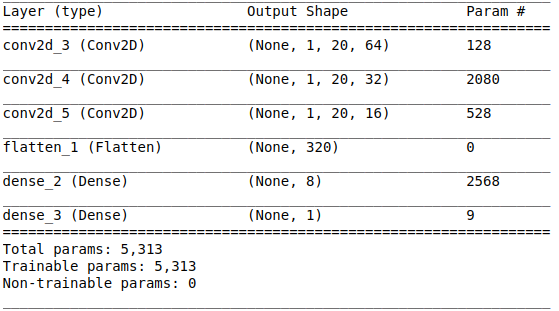
\includegraphics[width=0.8\textwidth]{others/cnn_summary.png}}%
  \caption{CNN Architecture}
  \label{fig:key}
\end{figure}

6 Experiments were conducted taking CNN model and we ran one of the experiments without applying any obersampling and smote with PCA taking 10 components. Rest of the 5 experiments were applying on oversampled and SMOTE balanced data with different feature selection techniques. The performance results are as follows:
 
%Please add the following packages if necessary:
%\usepackage{booktabs, multirow} % for borders and merged ranges
%\usepackage{soul}% for underlines
%\usepackage[table]{xcolor} % for cell colors
%\usepackage{changepage,threeparttable} % for wide tables
%If the table is too wide, replace \begin{table}[!htp]...\end{table} with
%\begin{adjustwidth}{-2.5 cm}{-2.5 cm}\centering\begin{threeparttable}[!htb]...\end{threeparttable}\end{adjustwidth}
\begin{table}[!htp]\centering
\caption{CNN Experiments Details}\label{tab: }
\scriptsize
\begin{tabular}{lrrrr}\toprule
Model Number &Feature Selection &No. of components &Oversampling and SMOTE \\
1 &N/A &N/A &yes \\\midrule
2 &SVD &10 &yes \\
3 &SVD &15 &yes \\
4 &\textbf{PCA} &\textbf{10} &\textbf{yes} \\
5 &PCA &10 &no \\
6 &PCA &15 &yes \\
\bottomrule
\end{tabular}
\end{table}

%Please add the following packages if necessary:
%\usepackage{booktabs, multirow} % for borders and merged ranges
%\usepackage{soul}% for underlines
%\usepackage[table]{xcolor} % for cell colors
%\usepackage{changepage,threeparttable} % for wide tables
%If the table is too wide, replace \begin{table}[!htp]...\end{table} with
%\begin{adjustwidth}{-2.5 cm}{-2.5 cm}\centering\begin{threeparttable}[!htb]...\end{threeparttable}\end{adjustwidth}
\begin{table}[!htp]\centering
\caption{CNN Model results}\label{tab: }
\scriptsize
\begin{tabular}{lrrrrr}\toprule
Model Number &FPA &CLC &Train Loss at last epoch(MSE) &Test Loss(MSE) \\
1 &0.484641 &0.4930281 &0.5649 &1.1203 \\\midrule
2 &0.4716726 &0.4800206 &0.094 &0.7005 \\
3 &NAN &NAN &3.5 &0.3652 \\
4 &\textbf{0.498646} &\textbf{0.507073} &\textbf{0.1769} &\textbf{0.7597} \\
5 &0.473417 &0.481844 &0.2426 &0.4125 \\
6 &0.478746 &0.487105 &0.1106 &0.743 \\
\bottomrule
\end{tabular}
\end{table}
 
Observing the results, we obtained undesired NAN values for FPA and CLC when we applied SVD and obtained 15 components. The best results were obtained when we ran the model with oversampled and SMOTE balanced data after applying PCA and obtaining 10 components. 

\subsection{LSTM}

Three different architectures were tried and they are as follows:
 \begin{itemize}
     \item Architecture 1: Three LSTM layers with decreasing output features and single dense layer at the end.
     \item Architecture 2: Five LSTM layers with decreasing output features and single dense layer at the end.
     \item Architecture 3: Seven LSTM layers with decreasing output features and single dense layer at the end.
 \end{itemize}
 
 The summaries of the three LSTM architectures tried as as follows:
 
 \begin{figure}
\makebox[\textwidth][c]{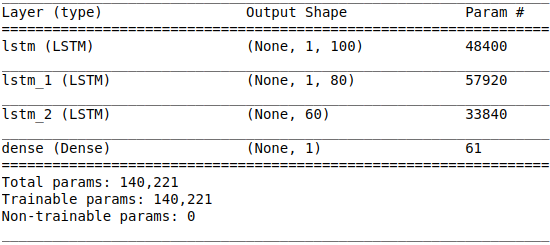
\includegraphics[width=0.8\textwidth]{others/LSTM_summary1.png}}%
  \caption{LSTM Architecture 1}
  \label{fig:key}
\end{figure}

\begin{figure}
\makebox[\textwidth][c]{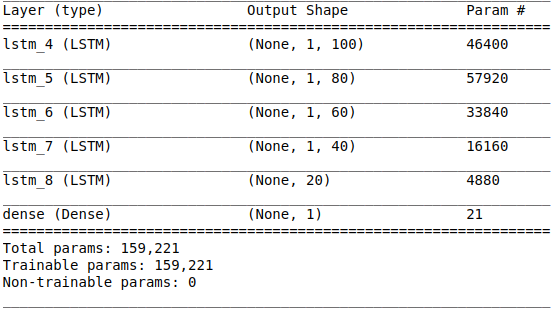
\includegraphics[width=0.8\textwidth]{others/LSTM_summary2.png}}%
  \caption{LSTM Architecture 2}
  \label{fig:key}
\end{figure}

\begin{figure}
\makebox[\textwidth][c]{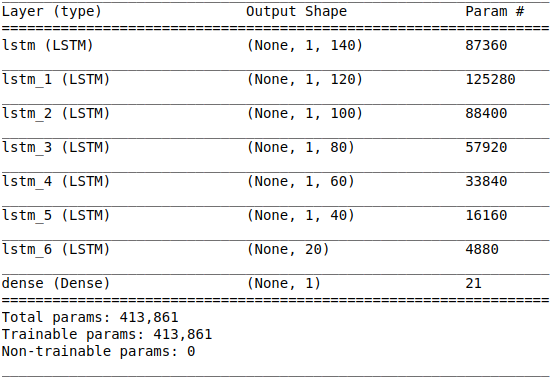
\includegraphics[width=0.8\textwidth]{others/LSTM_summary3.png}}%
  \caption{LSTM Architecture 3}
  \label{fig:key}
\end{figure}
 
Oversampling and SMOTE were applied to all the experiments involving the three LSTM models also. Info gain was taken as a feature selection criteria in one of the experiments. Considering the info gain, 9 features were selected. They are: CBO, RFC, Ce, LCOM3, LOC, DAM, MOA, MFA and CAM. The explanation of the following features are given in chapter 2.

The performance results are as follows:

%Please add the following packages if necessary:
%\usepackage{booktabs, multirow} % for borders and merged ranges
%\usepackage{soul}% for underlines
%\usepackage[table]{xcolor} % for cell colors
%\usepackage{changepage,threeparttable} % for wide tables
%If the table is too wide, replace \begin{table}[!htp]...\end{table} with
%\begin{adjustwidth}{-2.5 cm}{-2.5 cm}\centering\begin{threeparttable}[!htb]...\end{threeparttable}\end{adjustwidth}
\begin{table}[!htp]\centering
\caption{LSTM Experiments Details}\label{tab: }
\scriptsize
\begin{tabular}{lrrrr}\toprule
Model Number &Architecture Number &Feature Selection &No. of components \\
1 &1 &N/A &N/A \\\midrule
2 &1 &SVD &15 \\
3 &1 &SVD &10 \\
4 &1 &Info\_gain &9 Features selected \\
5 &1 &PCA &15 \\
6 &1 &PCA &10 \\
7 &\textbf{2} &\textbf{PCA} &\textbf{15} \\
8 &3 &PCA &15 \\
\bottomrule
\end{tabular}
\end{table}

%Please add the following packages if necessary:
%\usepackage{booktabs, multirow} % for borders and merged ranges
%\usepackage{soul}% for underlines
%\usepackage[table]{xcolor} % for cell colors
%\usepackage{changepage,threeparttable} % for wide tables
%If the table is too wide, replace \begin{table}[!htp]...\end{table} with
%\begin{adjustwidth}{-2.5 cm}{-2.5 cm}\centering\begin{threeparttable}[!htb]...\end{threeparttable}\end{adjustwidth}
\begin{table}[!htp]\centering
\caption{LSTM Model results}\label{tab: }
\scriptsize
\begin{tabular}{lrrrrr}\toprule
Model Number &FPA &CLC &Train Loss at last epoch(MSE) &Test Loss(MSE) \\
1 &0.4891348 &0.49753347 &0.9225 &1.3541 \\\midrule
2 &0.4854812 &0.4938745 &0.8029 &1.2402 \\
3 &0.48686993 &0.49526507 &0.7701 &1.2719 \\
4 &0.48584172 &0.494218 &0.9962 &1.421 \\
5 &0.49402896 &0.5024241 &0.7275 &1.2536 \\
6 &0.4832134 &0.4916067 &0.7384 &1.1761 \\
7 &\textbf{0.504664} &\textbf{0.5130555} &\textbf{0.741} &\textbf{1.2263} \\
8 &0.4919156 &0.5003081 &0.7219 &1.3139 \\
\bottomrule
\end{tabular}
\end{table}

From the table, we can observe that the best result was obtained from the LSTM model with architecture 2 when PCA was applied on the data and 15 components were obtained. The second best result was obtained from the architecture 1 of the LSTM models when PCA was obtained and 15 components were taken.

\subsection{RNN}

Three different architectures were tried and they are as follows:
 \begin{itemize}
     \item Architecture 1: Three RNN layers with decreasing output features and single dense layer at the end.
     \item Architecture 2: Five RNN layers with decreasing output features and single dense layer at the end.
     \item Architecture 3: Three RNN layers with decreasing output features and single dense layer at the end. This architecture is slightly less complex than the 1st RNN architecture.
 \end{itemize}
 
 The summaries of the three RNN architectures tried as as follows:
 
 \begin{figure}
\makebox[\textwidth][c]{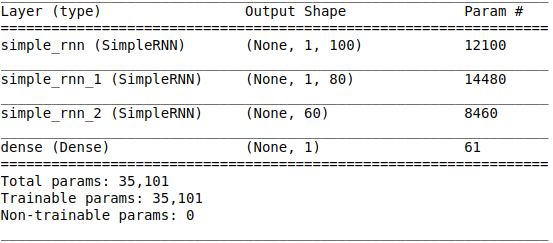
\includegraphics[width=0.8\textwidth]{others/rnn_summary1.png}}%
  \caption{RNN Architecture 1}
  \label{fig:key}
\end{figure}

\begin{figure}
\makebox[\textwidth][c]{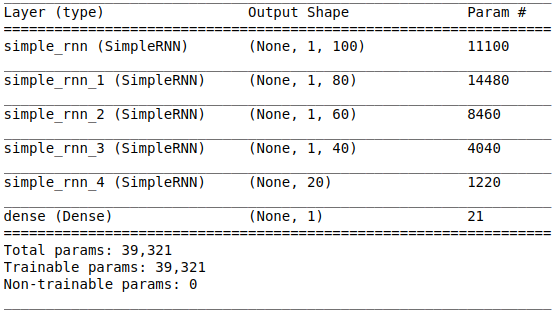
\includegraphics[width=0.8\textwidth]{others/rnn_summary2.png}}%
  \caption{RNN Architecture 2}
  \label{fig:key}
\end{figure}

\begin{figure}
\makebox[\textwidth][c]{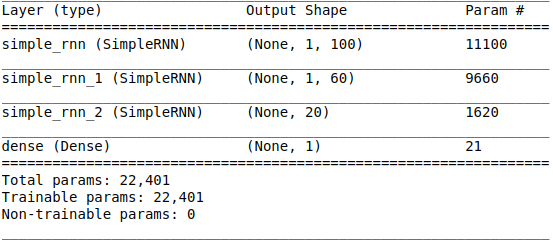
\includegraphics[width=0.8\textwidth]{others/rnn_summary3.png}}%
  \caption{RNN Architecture 3}
  \label{fig:key}
\end{figure}
 
8 experiments were performed on the RNN models of which in one experiment, we have not oversampled and SMOTE balanced the data. 

The performance results are as follows:

%Please add the following packages if necessary:
%\usepackage{booktabs, multirow} % for borders and merged ranges
%\usepackage{soul}% for underlines
%\usepackage[table]{xcolor} % for cell colors
%\usepackage{changepage,threeparttable} % for wide tables
%If the table is too wide, replace \begin{table}[!htp]...\end{table} with
%\begin{adjustwidth}{-2.5 cm}{-2.5 cm}\centering\begin{threeparttable}[!htb]...\end{threeparttable}\end{adjustwidth}
\begin{table}[!htp]\centering
\caption{RNN Experiments Details}\label{tab: }
\scriptsize
\begin{tabular}{lrrrrr}\toprule
Model Number &Architecture Number &Feature Selection &No. of components &Oversampling and SMOTE \\
1 &1 &N/A &N/A &yes \\\midrule
2 &\textbf{1} &\textbf{SVD} &\textbf{10} &\textbf{yes} \\
3 &1 &SVD &10 &no \\
4 &1 &SVD &15 &yes \\
5 &1 &PCA &10 &yes \\
6 &1 &PCA &15 &yes \\
7 &2 &SVD &10 &yes \\
8 &3 &SVD &10 &yes \\
\bottomrule
\end{tabular}
\end{table}

%Please add the following packages if necessary:
%\usepackage{booktabs, multirow} % for borders and merged ranges
%\usepackage{soul}% for underlines
%\usepackage[table]{xcolor} % for cell colors
%\usepackage{changepage,threeparttable} % for wide tables
%If the table is too wide, replace \begin{table}[!htp]...\end{table} with
%\begin{adjustwidth}{-2.5 cm}{-2.5 cm}\centering\begin{threeparttable}[!htb]...\end{threeparttable}\end{adjustwidth}
\begin{table}[!htp]\centering
\caption{RNN Model results}\label{tab: }
\scriptsize
\begin{tabular}{lrrrrr}\toprule
Model Number &FPA &CLC &Train Loss at last epoch(MSE) &Test Loss(MSE) \\
1 &0.49177 &0.50014 &0.8385 &1.3362 \\\midrule
2 &\textbf{0.50518} &\textbf{0.51357} &\textbf{0.6928} &\textbf{1.2263} \\
3 &0.49487 &0.5033 &0.3527 &0.3634 \\
4 &0.48322 &0.49161 &0.5944 &1.0027 \\
5 &0.48304 &0.49143 &0.7491 &1.1926 \\
6 &0.49248 &0.50087 &0.5342 &0.9949 \\
7 &0.49188 &0.50027 &0.644 &1.1513 \\
8 &0.47143 &0.479826 &0.6852 &1.156 \\
\bottomrule
\end{tabular}
\end{table}

From the table, we can observe that the best result was obtained when SVD was applied on oversampled and SMOTE balanced data and 10 components were selected. 

The training curve of the best performing model among the 32 experiments is plotted using tensorboard and it is visualized as follows:

 \begin{figure}
\makebox[\textwidth][c]{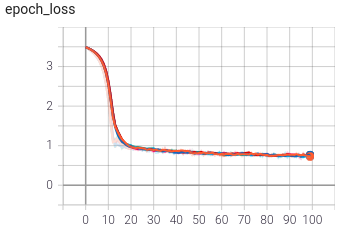
\includegraphics[width=0.8\textwidth]{others/epoch_loss.png}}%
  \caption{Training curve}
  \label{fig:key}
\end{figure}

